\large

{\sffamily\Large\bfseries What will you learn in this class?}

You will learn how to write programs that run fast and use computers
efficiently.

\textbf{Pop Quiz:} \$400 at your favorite electronics retailer
buys you a parallel computer that will do
$4\cdot 10^{12}$ floating point operations (``flops'') per second,
but only load $5\cdot 10^{10}$ values from memory in the same
amount of time. How do you use such a machine well?

What to expect:
\vspace{-0.5em}
\begin{itemize}
\setlength{\itemsep}{-1mm}
  \item Basic processor architecture\\
    Performance of sequential code
  \item Why go parallel? Forms of parallelism
  \item Shared Memory and \textbf{OpenMP}
  \item Tools and Debuggers
  \item \textbf{GPUs} and \textbf{OpenCL}
  \item Distributed Memory and \textbf{MPI}
  \item Common Patterns in Parallel Algorithms
\end{itemize}

\columnbreak
{\sffamily\Large\bfseries Who should take this class?}

\vspace{-0.5em}
\begin{itemize}
\setlength{\itemsep}{-1mm}
  \item Graduate students
  \item Advanced undergrads
  \item Researchers
\end{itemize}
\vspace{-0.5em}
If you have a computation-heavy problem that you would like to go
faster, you're especially welcome.

\emph{Prerequisites:} Working knowledge of C\\
\emph{Assessment:} Weekly homework, final
project.

We're looking forward to seeing you in the fall!

\hfill \emph{Marsha Berger} \hfill \emph{Andreas Klöckner}

\centering
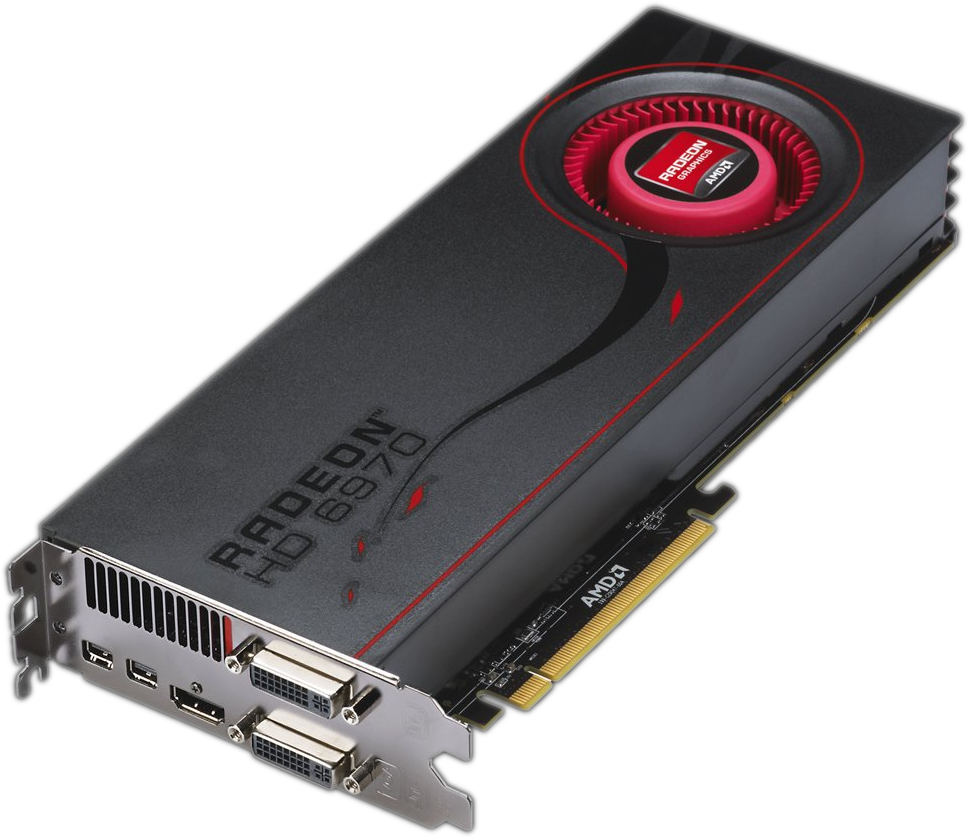
\includegraphics[width=0.6\columnwidth]{amd-6970.png}
